% Gerado automaticamente. No preambulo do documento use:
% \usepackage{pgfplots}
% \pgfplotsset{compat=1.18}
\definecolor{plotblue}{HTML}{2563EB}
\definecolor{plotorange}{HTML}{D97706}
\definecolor{plotgreen}{HTML}{059669}
\definecolor{plotpurple}{HTML}{7C3AED}
\definecolor{plotgray}{HTML}{374151}
\definecolor{plotred}{HTML}{DC2626}
\definecolor{plotteal}{HTML}{0F766E}
\definecolor{plotslate}{HTML}{64748B}

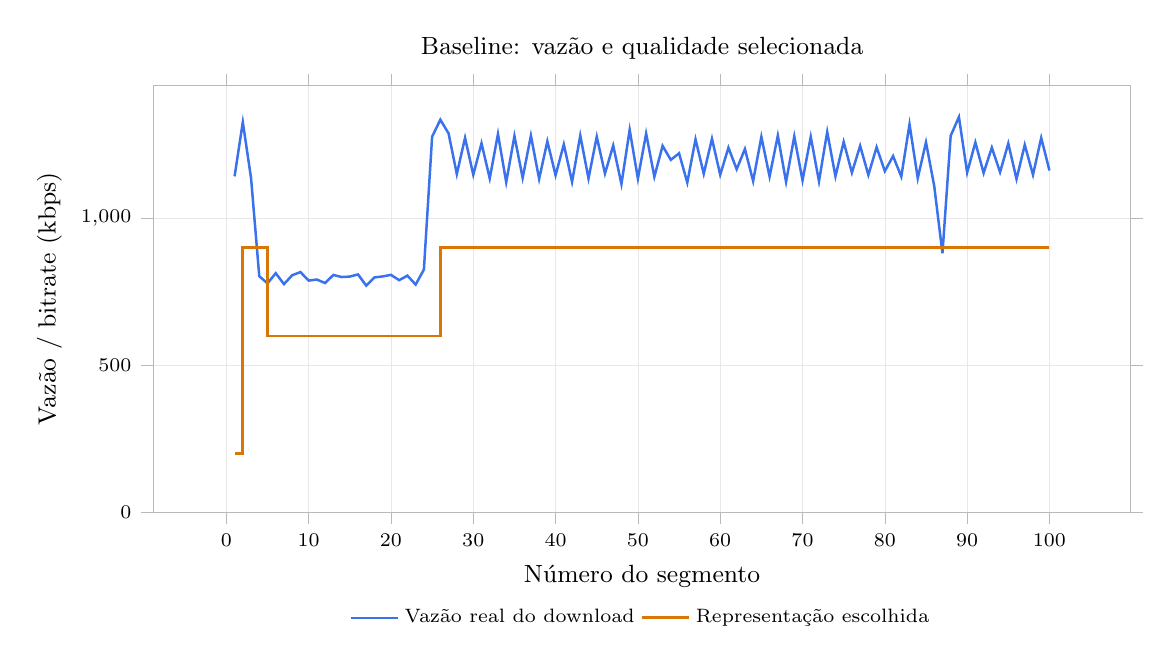
\begin{tikzpicture}
\begin{axis}[
    title={Baseline: vazão e qualidade selecionada},
    xlabel={Número do segmento},
    ylabel={Vazão / bitrate (kbps)},
    width=14cm,
    height=7cm,
    grid=major,
    grid style={line width=.12pt, draw=gray!18},
    axis line style={draw=gray!55},
    tick style={draw=gray!55},
    tick align=outside,
    title style={font=\small},
    label style={font=\small},
    tick label style={font=\scriptsize},
    legend cell align={left},
    legend style={at={(0.5,-0.20)}, anchor=north, legend columns=3, draw=none, font=\scriptsize},
    ymin=0,
    ymax=1453.73
]
\addplot+[plotblue, line width=0.9pt, mark=none, opacity=0.9] coordinates {
(1,1143.95)
(2,1328.54)
(3,1138.18)
(4,803.55)
(5,779.31)
(6,813.9)
(7,776.71)
(8,806.99)
(9,817.64)
(10,788.74)
(11,792.33)
(12,780.3)
(13,808.01)
(14,800.8)
(15,802.36)
(16,809.8)
(17,771.28)
(18,799.55)
(19,802.93)
(20,808.17)
(21,790.17)
(22,805.51)
(23,775.11)
(24,826.37)
(25,1279.19)
(26,1336.91)
(27,1290.04)
(28,1151.62)
(29,1275.14)
(30,1149.32)
(31,1256.44)
(32,1136.78)
(33,1288.3)
(34,1123.63)
(35,1281.4)
(36,1138.63)
(37,1282.65)
(38,1134.98)
(39,1263.17)
(40,1147.59)
(41,1252.75)
(42,1125.01)
(43,1282.76)
(44,1136.76)
(45,1279.06)
(46,1153.33)
(47,1249.03)
(48,1117.68)
(49,1302.46)
(50,1136.21)
(51,1289.81)
(52,1142.6)
(53,1247.8)
(54,1200.18)
(55,1222.35)
(56,1122.79)
(57,1270.05)
(58,1152.65)
(59,1272.04)
(60,1149.34)
(61,1241.64)
(62,1168.11)
(63,1237.03)
(64,1127.87)
(65,1278.56)
(66,1143.15)
(67,1282.93)
(68,1125.11)
(69,1279.8)
(70,1130.02)
(71,1278.61)
(72,1127.05)
(73,1295.46)
(74,1143.96)
(75,1261.52)
(76,1156.48)
(77,1247.96)
(78,1148.67)
(79,1243.1)
(80,1161.66)
(81,1212.87)
(82,1143.09)
(83,1321.32)
(84,1137.56)
(85,1259.92)
(86,1111.08)
(87,881.67)
(88,1282.07)
(89,1346.05)
(90,1156.73)
(91,1259.5)
(92,1155.33)
(93,1241.68)
(94,1158.25)
(95,1256.09)
(96,1134.58)
(97,1251.19)
(98,1149.3)
(99,1275)
(100,1163.95)
};
\addlegendentry{Vazão real do download}
\addplot+[plotorange, const plot, line width=1.05pt, mark=none] coordinates {
(1,200)
(2,900)
(3,900)
(4,900)
(5,600)
(6,600)
(7,600)
(8,600)
(9,600)
(10,600)
(11,600)
(12,600)
(13,600)
(14,600)
(15,600)
(16,600)
(17,600)
(18,600)
(19,600)
(20,600)
(21,600)
(22,600)
(23,600)
(24,600)
(25,600)
(26,900)
(27,900)
(28,900)
(29,900)
(30,900)
(31,900)
(32,900)
(33,900)
(34,900)
(35,900)
(36,900)
(37,900)
(38,900)
(39,900)
(40,900)
(41,900)
(42,900)
(43,900)
(44,900)
(45,900)
(46,900)
(47,900)
(48,900)
(49,900)
(50,900)
(51,900)
(52,900)
(53,900)
(54,900)
(55,900)
(56,900)
(57,900)
(58,900)
(59,900)
(60,900)
(61,900)
(62,900)
(63,900)
(64,900)
(65,900)
(66,900)
(67,900)
(68,900)
(69,900)
(70,900)
(71,900)
(72,900)
(73,900)
(74,900)
(75,900)
(76,900)
(77,900)
(78,900)
(79,900)
(80,900)
(81,900)
(82,900)
(83,900)
(84,900)
(85,900)
(86,900)
(87,900)
(88,900)
(89,900)
(90,900)
(91,900)
(92,900)
(93,900)
(94,900)
(95,900)
(96,900)
(97,900)
(98,900)
(99,900)
(100,900)
};
\addlegendentry{Representação escolhida}
\end{axis}
\end{tikzpicture}
